\documentclass{article}
\usepackage[utf8]{inputenc}
\usepackage[spanish]{babel}
\usepackage{listings}
\usepackage{subfigure}
\usepackage{graphicx}
\usepackage{url}
\usepackage{multirow}
\usepackage{multicol}
\usepackage{color}
\usepackage{booktabs}
\usepackage{float}
\usepackage{amsmath}
%\usepackage{verbatim}
\usepackage{hyperref}
\hypersetup{
    colorlinks=true,
    linkcolor=blue,
    filecolor=magenta,      
    urlcolor=cyan,
}
\usepackage[margin=3cm,twoside]{geometry} 
\setlength{\parindent}{0pt}
\setlength{\parskip}{1em}
\usepackage{fancyvrb}





\definecolor{mygreen}{rgb}{0,0.6,0}
\definecolor{mygray}{rgb}{0.5,0.5,0.5}
\definecolor{mymauve}{rgb}{0.58,0,0.82}
\lstset{ 
  backgroundcolor=\color{white},   % choose the background color; you must add \usepackage{color} or \usepackage{xcolor}; should come as last argument
  basicstyle=\footnotesize,        % the size of the fonts that are used for the code
  breakatwhitespace=false,         % sets if automatic breaks should only happen at whitespace
  breaklines=true,                 % sets automatic line breaking
  captionpos=b,                    % sets the caption-position to bottom
  commentstyle=\color{mygreen},    % comment style
  deletekeywords={...},            % if you want to delete keywords from the given language
  escapeinside={\%*}{)},          % if you want to add LaTeX within your code
  extendedchars=true,              % lets you use non-ASCII characters; for 8-bits encodings only, does not work with UTF-8
  firstnumber=1,                % start line enumeration with line 1000
  frame=single,	                   % adds a frame around the code
  keepspaces=true,                 % keeps spaces in text, useful for keeping indentation of code (possibly needs columns=flexible)
  keywordstyle=\color{blue},       % keyword style
  language=Octave,                 % the language of the code
  morekeywords={*,...},            % if you want to add more keywords to the set
  numbers=left,                    % where to put the line-numbers; possible values are (none, left, right)
  numbersep=5pt,                   % how far the line-numbers are from the code
  numberstyle=\tiny\color{mygray}, % the style that is used for the line-numbers
  rulecolor=\color{black},         % if not set, the frame-color may be changed on line-breaks within not-black text (e.g. comments (green here))
  showspaces=false,                % show spaces everywhere adding particular underscores; it overrides 'showstringspaces'
  showstringspaces=false,          % underline spaces within strings only
  showtabs=false,                  % show tabs within strings adding particular underscores
  stepnumber=1,                    % the step between two line-numbers. If it's 1, each line will be numbered
  stringstyle=\color{mymauve},     % string literal style
  tabsize=2,	                   % sets default tabsize to 2 spaces
  title=\lstname                  % show the filename of files included with \lstinputlisting; also try caption instead of title
}
\usepackage{etoolbox}
\makeatletter
\providecommand{\subtitle}[1]{% add subtitle to \maketitle
  \apptocmd{\@title}{\par {\large #1 \par}}{}{}
}
\RecustomVerbatimCommand{\VerbatimInput}{VerbatimInput}%
{fontsize=\footnotesize,
	%
	frame=lines,  % top and bottom rule only
	framesep=2em, % separation between frame and text
	rulecolor=\color{mygreen},
	%
	label=\fbox{\color{black} summary.txt},
	labelposition=topline,
	%
	commandchars=\|\(\), % escape character and argument delimiters for
	% commands within the verbatim
	%commentchar=*        % comment character
}
\renewcommand{\theenumi}{\roman{enumi}}
\newtheorem{teor}{Teorema}
\makeatother
\title{Tarea 10 de Modelos Probabilistas Aplicados}
\subtitle{Ejercicios}

\author{5271}
\date{\today}

\begin{document}

\maketitle
\section{Introducción}
En este documento se presentan los resultados de varios ejercicios del libro ``\textit{Introduction to Probability}''\cite{libProba} encontrados de forma analítica, así como los resultados alcanzados numéricamente mediante simulación.
\section{Valor esperado}

Ahora para variables aleatorias discretas el valor esperado es:
\begin{equation}\label{eq:3}
 E[X] = \sum_{x \in \Omega} x
	      \times P(X = x).   
\end{equation}
\section{Ejercicio 6 de la página 247}
\emph{A die is rolled twice. Let $X$ denote the sum of the two numbers that turn up, and Y the difference of the numbers (specifically, the number on the first roll minus the number on the second). Show that $E(X Y) = E(X)E(Y )$. Are $X$ and $Y$ independent?}


\subsection{$X = a + b$}
Sea $X = a + b$ donde $a$ es el valor del primer tiro y $b$ el segundo, se tiene:
$ X =$ 2--12. La frecuencia de los valores de $X$ se muestran en el cuadro \ref{tab:1} de la página \pageref{tab:1}.

\begin{table}[H]
  \centering
  \caption{Frecuencia de valores de $X$}
    \begin{tabular}{rrr}
    \toprule
    \multicolumn{1}{p{5.39em}}{\textbf{Posibles valores de \textit{\textbf{x}}}} & \multicolumn{1}{l}{\textbf{frecuencia  \textit{\textbf{(x)}}}} & \multicolumn{1}{l}{\textit{\textbf{P(X = x)}}} \\
    \midrule
    2     & 1     & 0.028 \\
    3     & 2     & 0.056 \\
    4     & 3     & 0.083 \\
    5     & 4     & 0.111 \\
    6     & 5     & 0.139 \\
    7     & 6     & 0.167 \\
    8     & 5     & 0.139 \\
    9     & 4     & 0.111 \\
    10    & 3     & 0.083 \\
    11    & 2     & 0.056 \\
    12    & 1     & 0.028 \\
    \bottomrule
    \end{tabular}%
  \label{tab:1}%
\end{table}%

Del cuadro \ref{tab:1} podemos obtener que:
\begin{equation}
 P(X = x_{i}) = \frac{\text{frecuencia de $x_{i}$} }{36}.   
\end{equation}
Sustituyendo en la ecuación \ref{eq:3}
\begin{equation}
\begin{array}{ll}
   E[X] &= \sum_{i=1}^{11} x_{i}  \times P(X=x_{i})\\
   &\\
   E[X] & = 7.
  \end{array}
\end{equation}
Para la comprobación y mejor entendimiento del resultado obtenido se realiza una simulación de la variable aleatoria $X = a + b$, la misma es realizada en R \cite{R} como se muestra en el código \ref{cod:1} a continuación.
\begin{center}
\lstinputlisting[ language=R, firstline=3, lastline=18]{Tarea10.R}
\label{cod:1}
\end{center}
Los valores para $X$ son almacenados en un \textit{dataframe}, como se muestra en el cuadro \ref{tab:s} de la página \pageref{tab:s}, al aplicarle la función \textit{summary} de R al \textit{dataframe} se obtiene los siguientes valores.  
\VerbatimInput{suma.txt}
En los valores obtenidos se puede observar que la media es igual a 6.848 por lo que se puede decir que el valor promedio obtenido es igual a la $E[X]$, además coincide con la mediana que es el valor con mayor frecuencia de ocurrencia de $X$ como se muestra en la figura \ref{fig:s} de la página \pageref{fig:s}. Para mejor visualización del experimento se puede ver la figura  \href{https://github.com/Albertomnoa/Tareas_MPA/blob/master/Tarea10/gif/suma.gif}{$X = (a+b)$.gif}, donde se observa el progreso de los lanzamientos.

\begin{table}[H]
  \centering
  \caption{fragmento de \textit{dataframe} de la variable aleatoria $X = a + b$}
    \begin{tabular}{rr}
    \toprule
    \multicolumn{1}{c}{Lanzamientos} & \multicolumn{1}{c}{x} \\
    \midrule
    1     & 6 \\
    2     & 11 \\
    3     & 6 \\
    4     & 9 \\
    5     & 4 \\
    161   & 7 \\
    162   & 3 \\
    163   & 6 \\
    164   & 7 \\
    165   & 8 \\
    996   & 6 \\
    997   & 9 \\
    998   & 11 \\
    999   & 11 \\
    1000  & 5 \\
    \bottomrule
    \end{tabular}%
  \label{tab:s}%
\end{table}%

\begin{figure}[H]
\centering
\subfigure[Histograma de frecuencia de la variable aleatoria $X$]{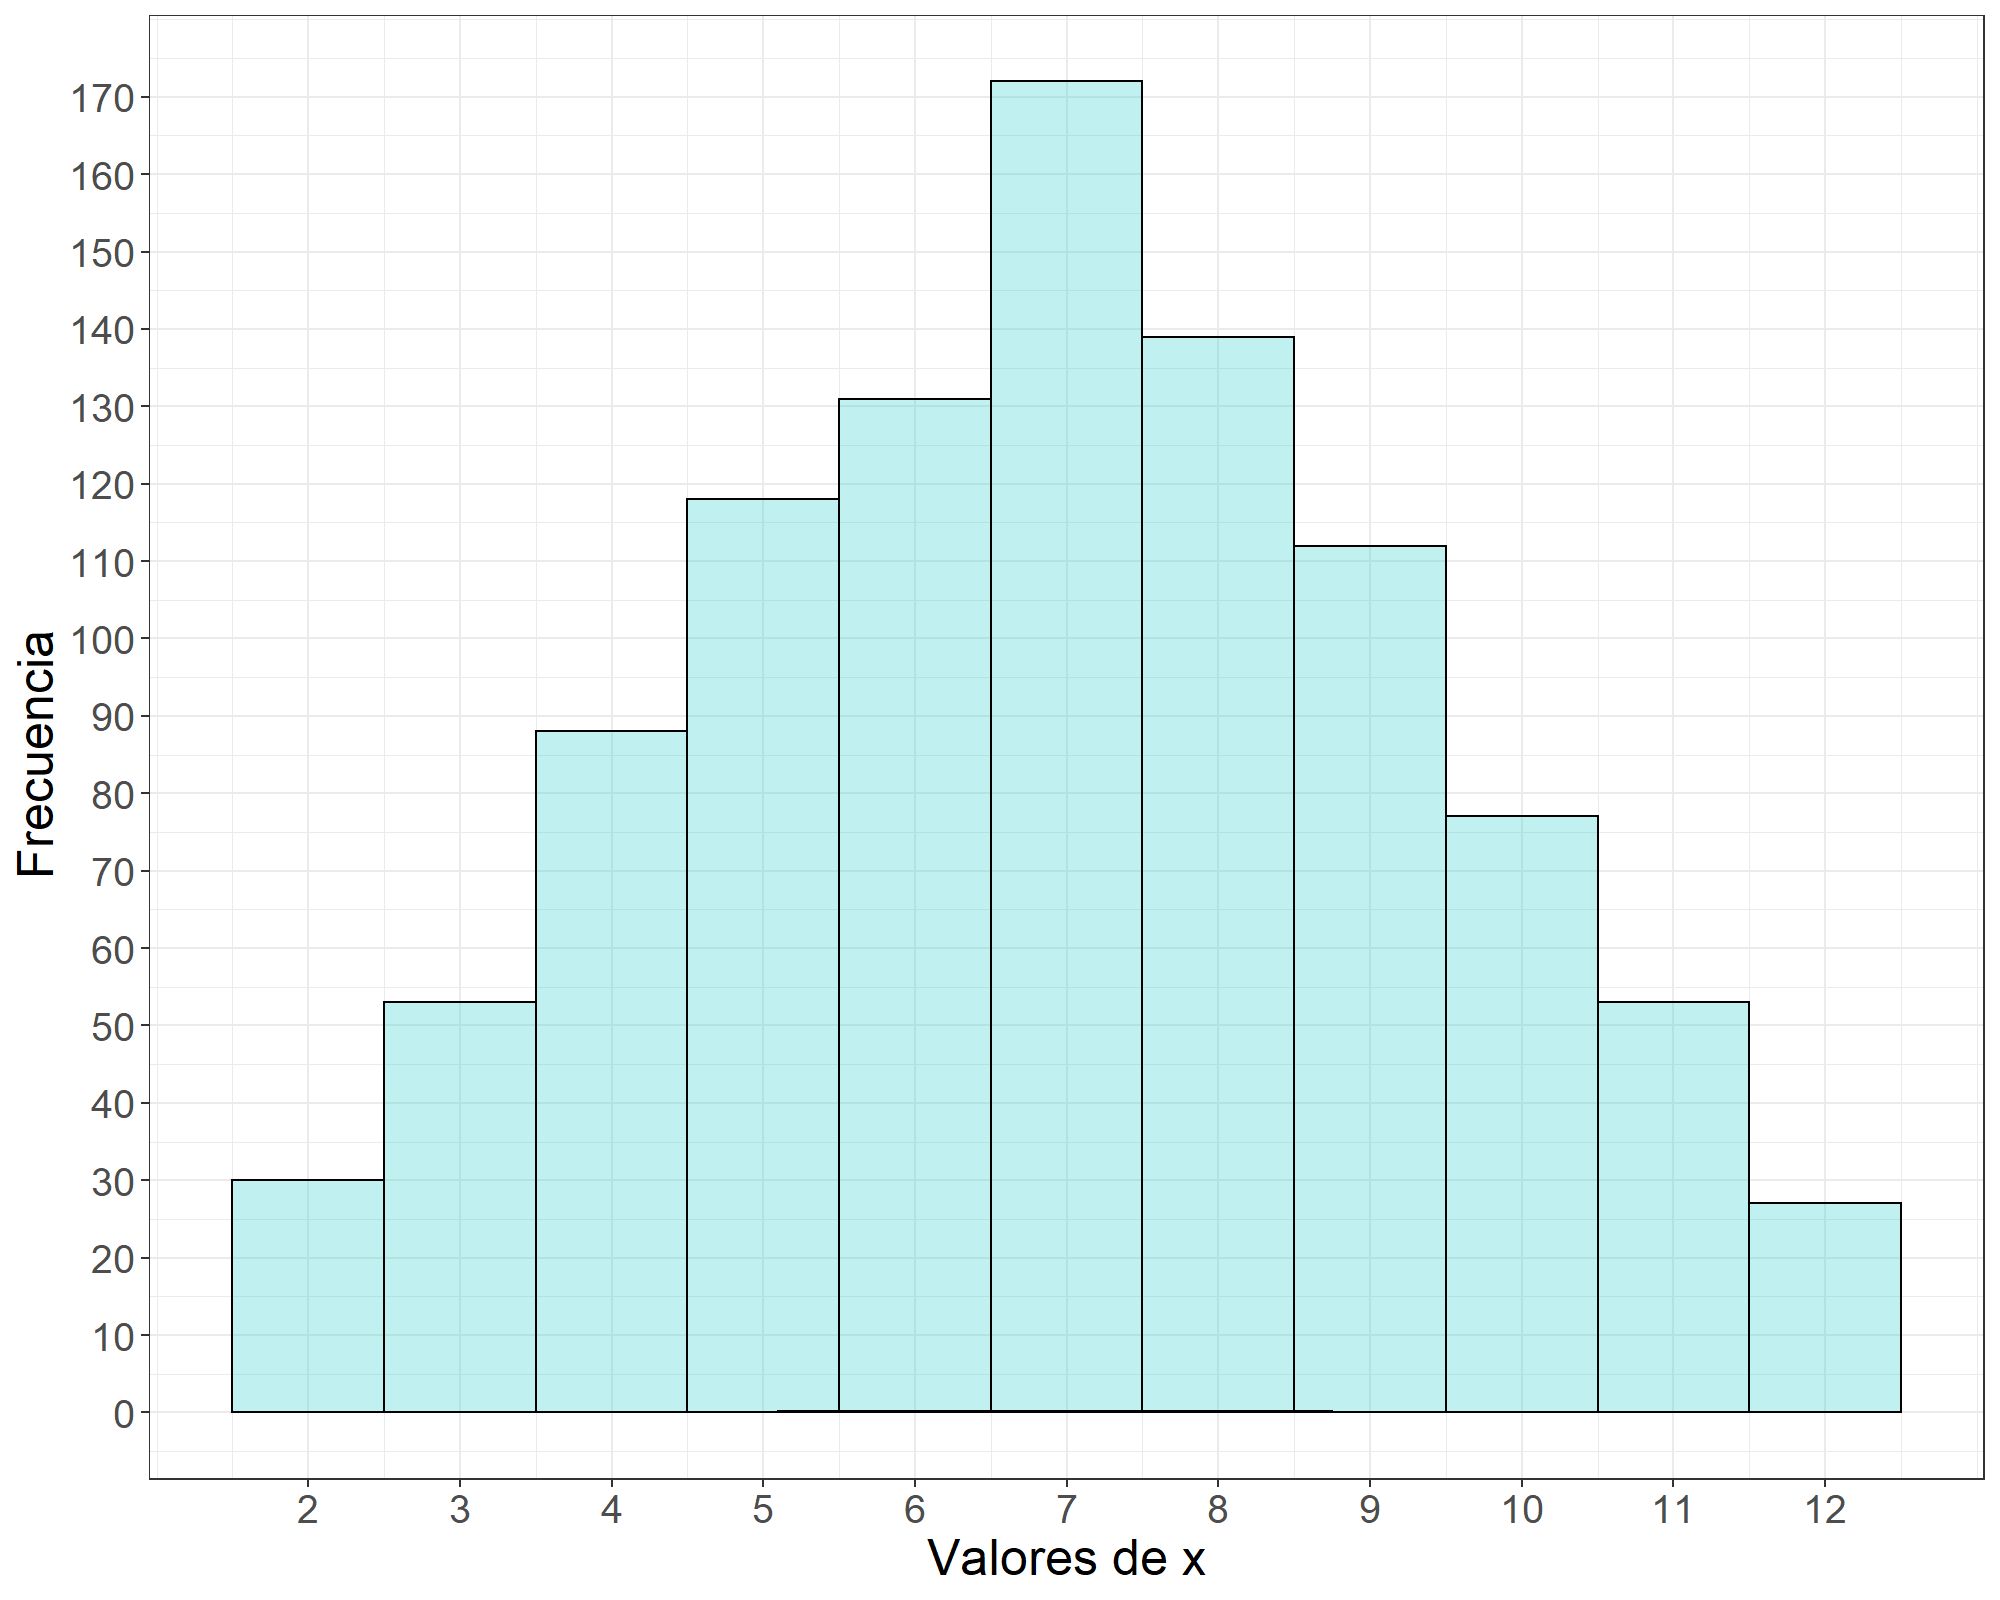
\includegraphics[scale=0.30]{figuras/sumas.png}}
\label{fig:a}
\centering
\subfigure[Histograma de densidad de la variable aleatoria $X$]{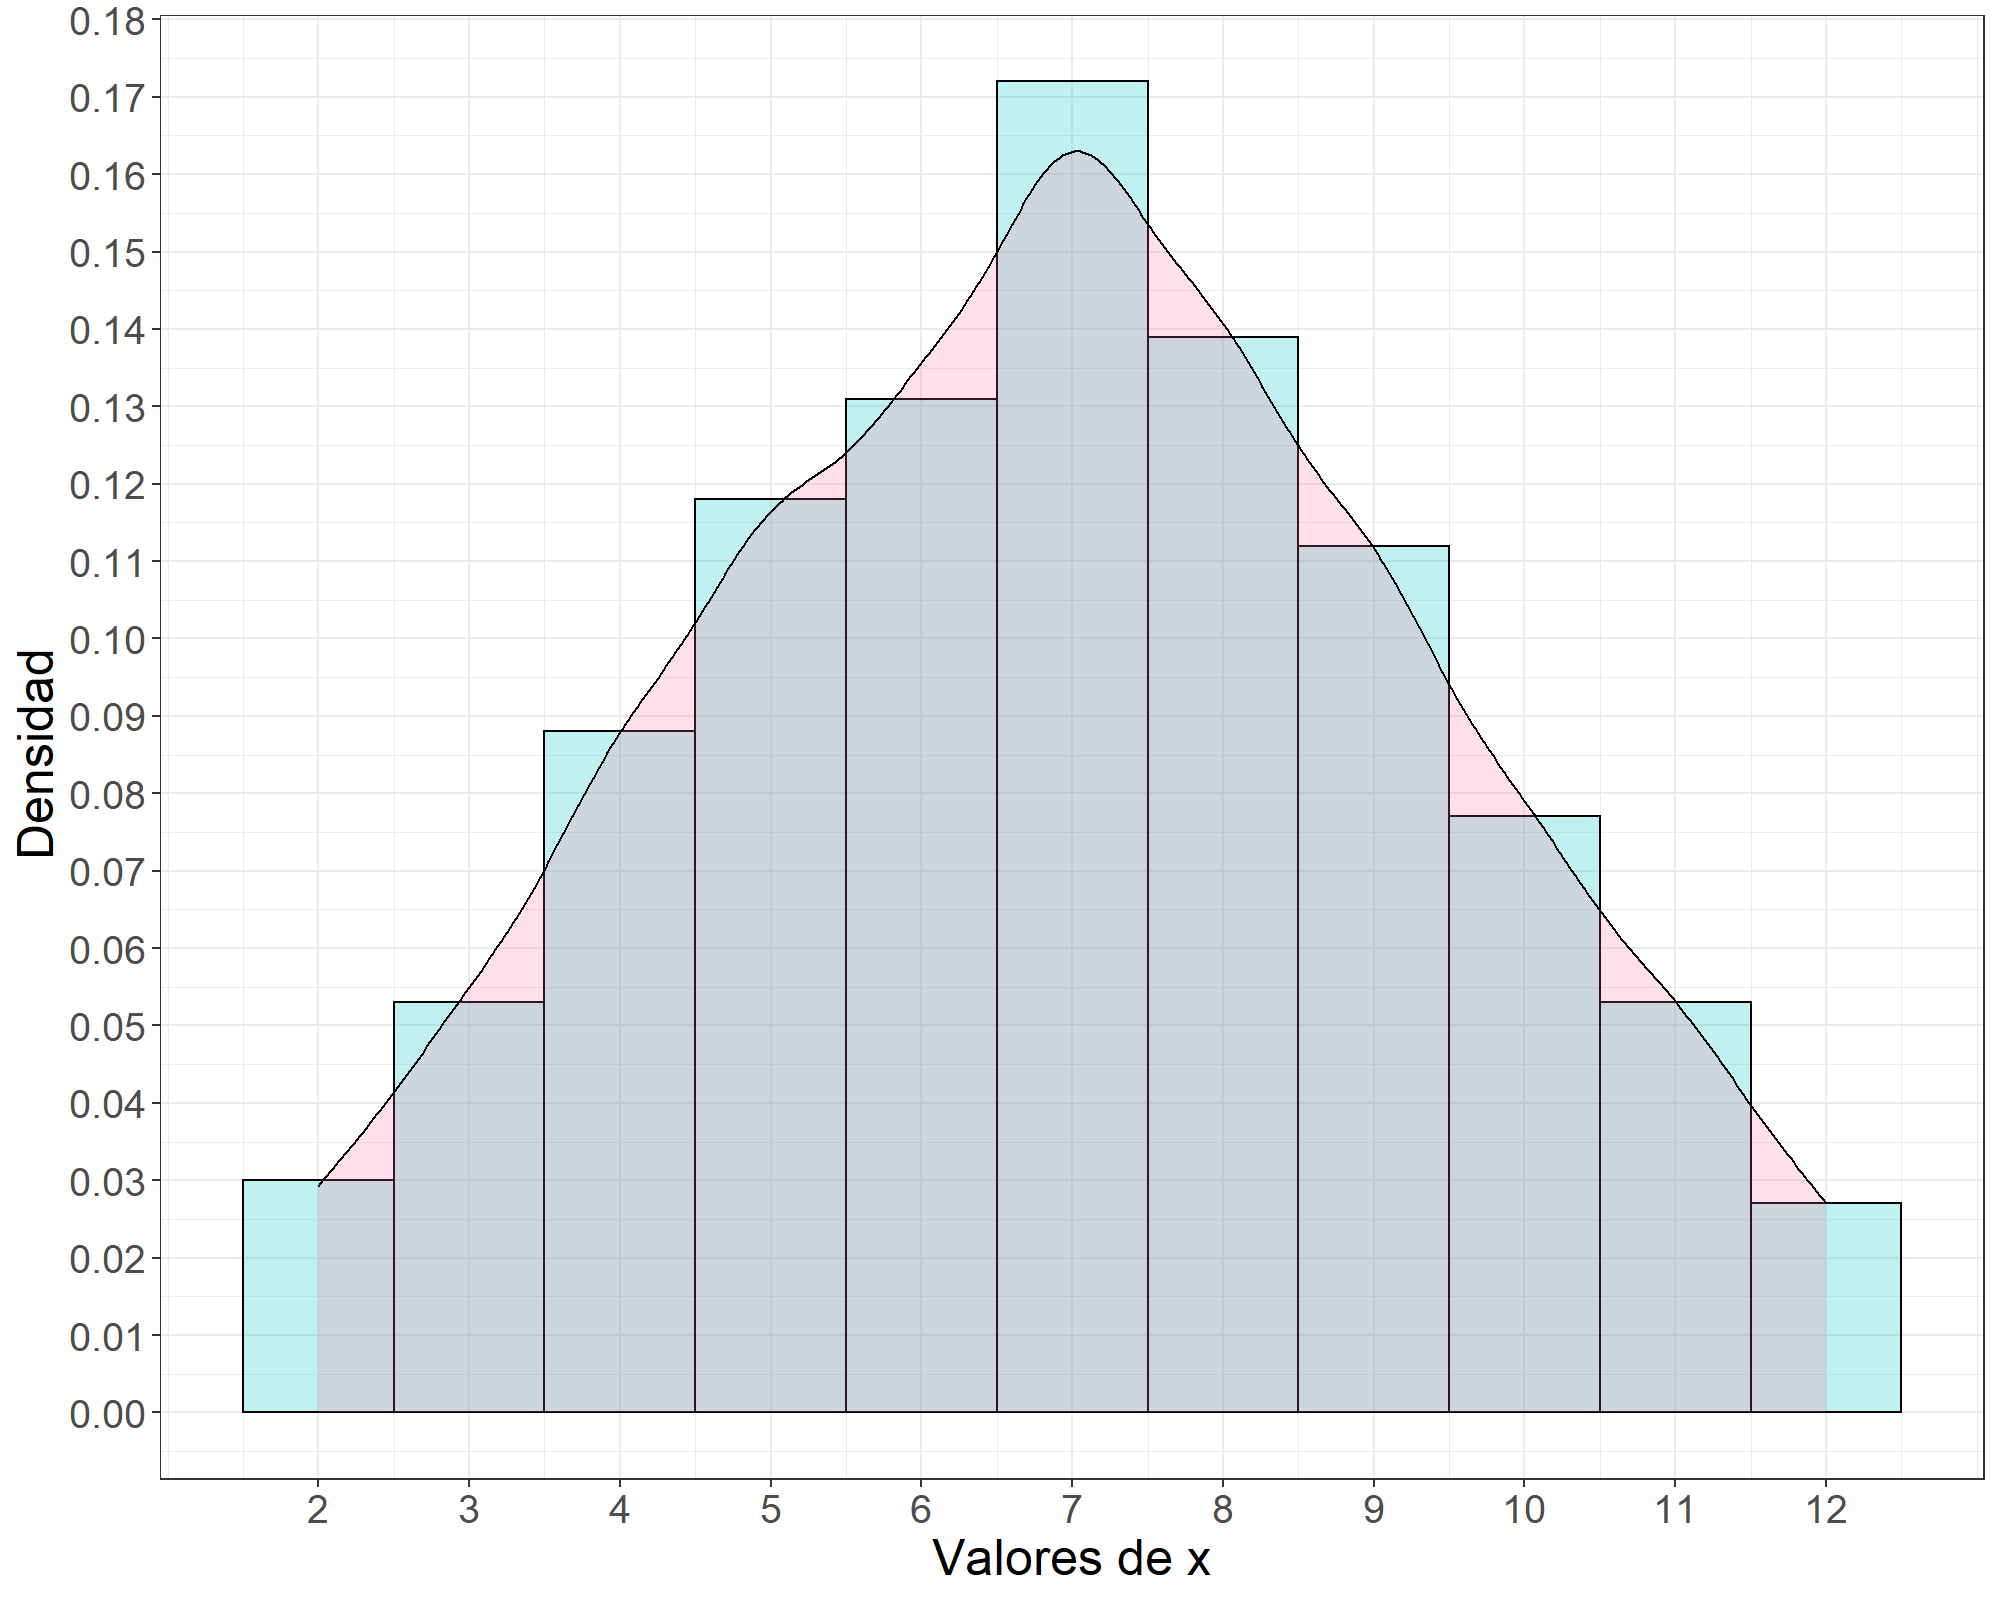
\includegraphics[scale=0.30]{figuras/dsumas.png}}
\label{fig:s}
\centering
\caption{Histogramas de la variable aleatoria $X= a + b$ }
\label{fig:1} 
\end{figure}

\subsection{$Y = a - b$}
Análogamente, sea $Y= a-b$. De $Y$ se obtiene los valores que muestra el cuadro \ref{tab:2} de la página \pageref{tab:2}.

% Table generated by Excel2LaTeX from sheet 'Fsum'
\begin{table}[H]
  \centering
  \caption{Frecuencia de valores de $X$ }
    \begin{tabular}{rrr}
    \toprule
    \multicolumn{1}{p{5.39em}}{\textbf{Posibles valores de \textit{\textbf{x}}}} & \multicolumn{1}{l}{\textbf{frecuencia  \textit{\textbf{(x)}}}}  & \multicolumn{1}{l}{\textit{\textbf{P(X = x)}}} \\
    \midrule
    -5    & 1     & 0.028 \\
    -4    & 2     & 0.056 \\
    -3    & 3     & 0.083 \\
    -2    & 4     & 0.111 \\
    -1    & 5     & 0.139 \\
    0     & 6     & 0.167 \\
    1     & 5     & 0.139 \\
    2     & 4     & 0.111 \\
    3     & 3     & 0.083 \\
    4     & 2     & 0.056 \\
    5     & 1     & 0.028 \\
    \bottomrule
    \end{tabular}%
  \label{tab:2}%
\end{table}%
Sustituyendo en la ecuación \ref{eq:3}
\begin{equation}
\begin{array}{ll}
   E[X] &= \sum_{i=1}^{11} x_{i}  \times P(X=x_{i})\\
   &\\
   E[X] & = 0.
  \end{array}
\end{equation}
Al comprobar con la simulación de la variable aleatoria $X = a - b$, los valores para $X$ son almacenados en un \textit{dataframe}, como se muestra en el cuadro \ref{tab:r} de la página \pageref{tab:r}, al aplicarle la función \textit{summary} de R al \textit{dataframe} se obtiene los siguientes valores.  
\VerbatimInput{resta.txt}

\begin{table}[H]
  \centering
  \caption{Fragmento de \textit{dataframe} de la variable aleatoria $$Y = a - b$$ }
    \begin{tabular}{rr}
    \toprule
    \multicolumn{1}{l}{Lanzamientos} & \multicolumn{1}{c}{y} \\
    \midrule
    1     & -4 \\
    2     & -1 \\
    3     & -2 \\
    4     & -3 \\
    5     & 2 \\
    201   & -3 \\
    202   & 0 \\
    203   & 1 \\
    204   & 0 \\
    205   & 5 \\
    996   & 2 \\
    997   & -1 \\
    998   & 1 \\
    999   & -1 \\
    1000  & -1 \\
    \bottomrule
    \end{tabular}%
  \label{tab:r}%
\end{table}%
En los valores obtenidos se puede observar que la media es igual a -0.082 por lo que se puede decir que el valor promedio obtenido es igual a la $E[Y]$, además coincide con la mediana que es el valor con mayor frecuencia de ocurrencia de $Y$ como se muestra en la figura \ref{fig:2} de la página \pageref{fig:2}. Para mejor visualización del experimento se puede ver la figura  \href{https://github.com/Albertomnoa/Tareas_MPA/blob/master/Tarea10/gif/resta.gif}{$Y = (a - b)$.gif}, donde se observa el progreso de los lanzamientos.

\begin{figure}[H]
\centering
\subfigure[Histograma de frecuencia de la variable aleatoria $Y$]{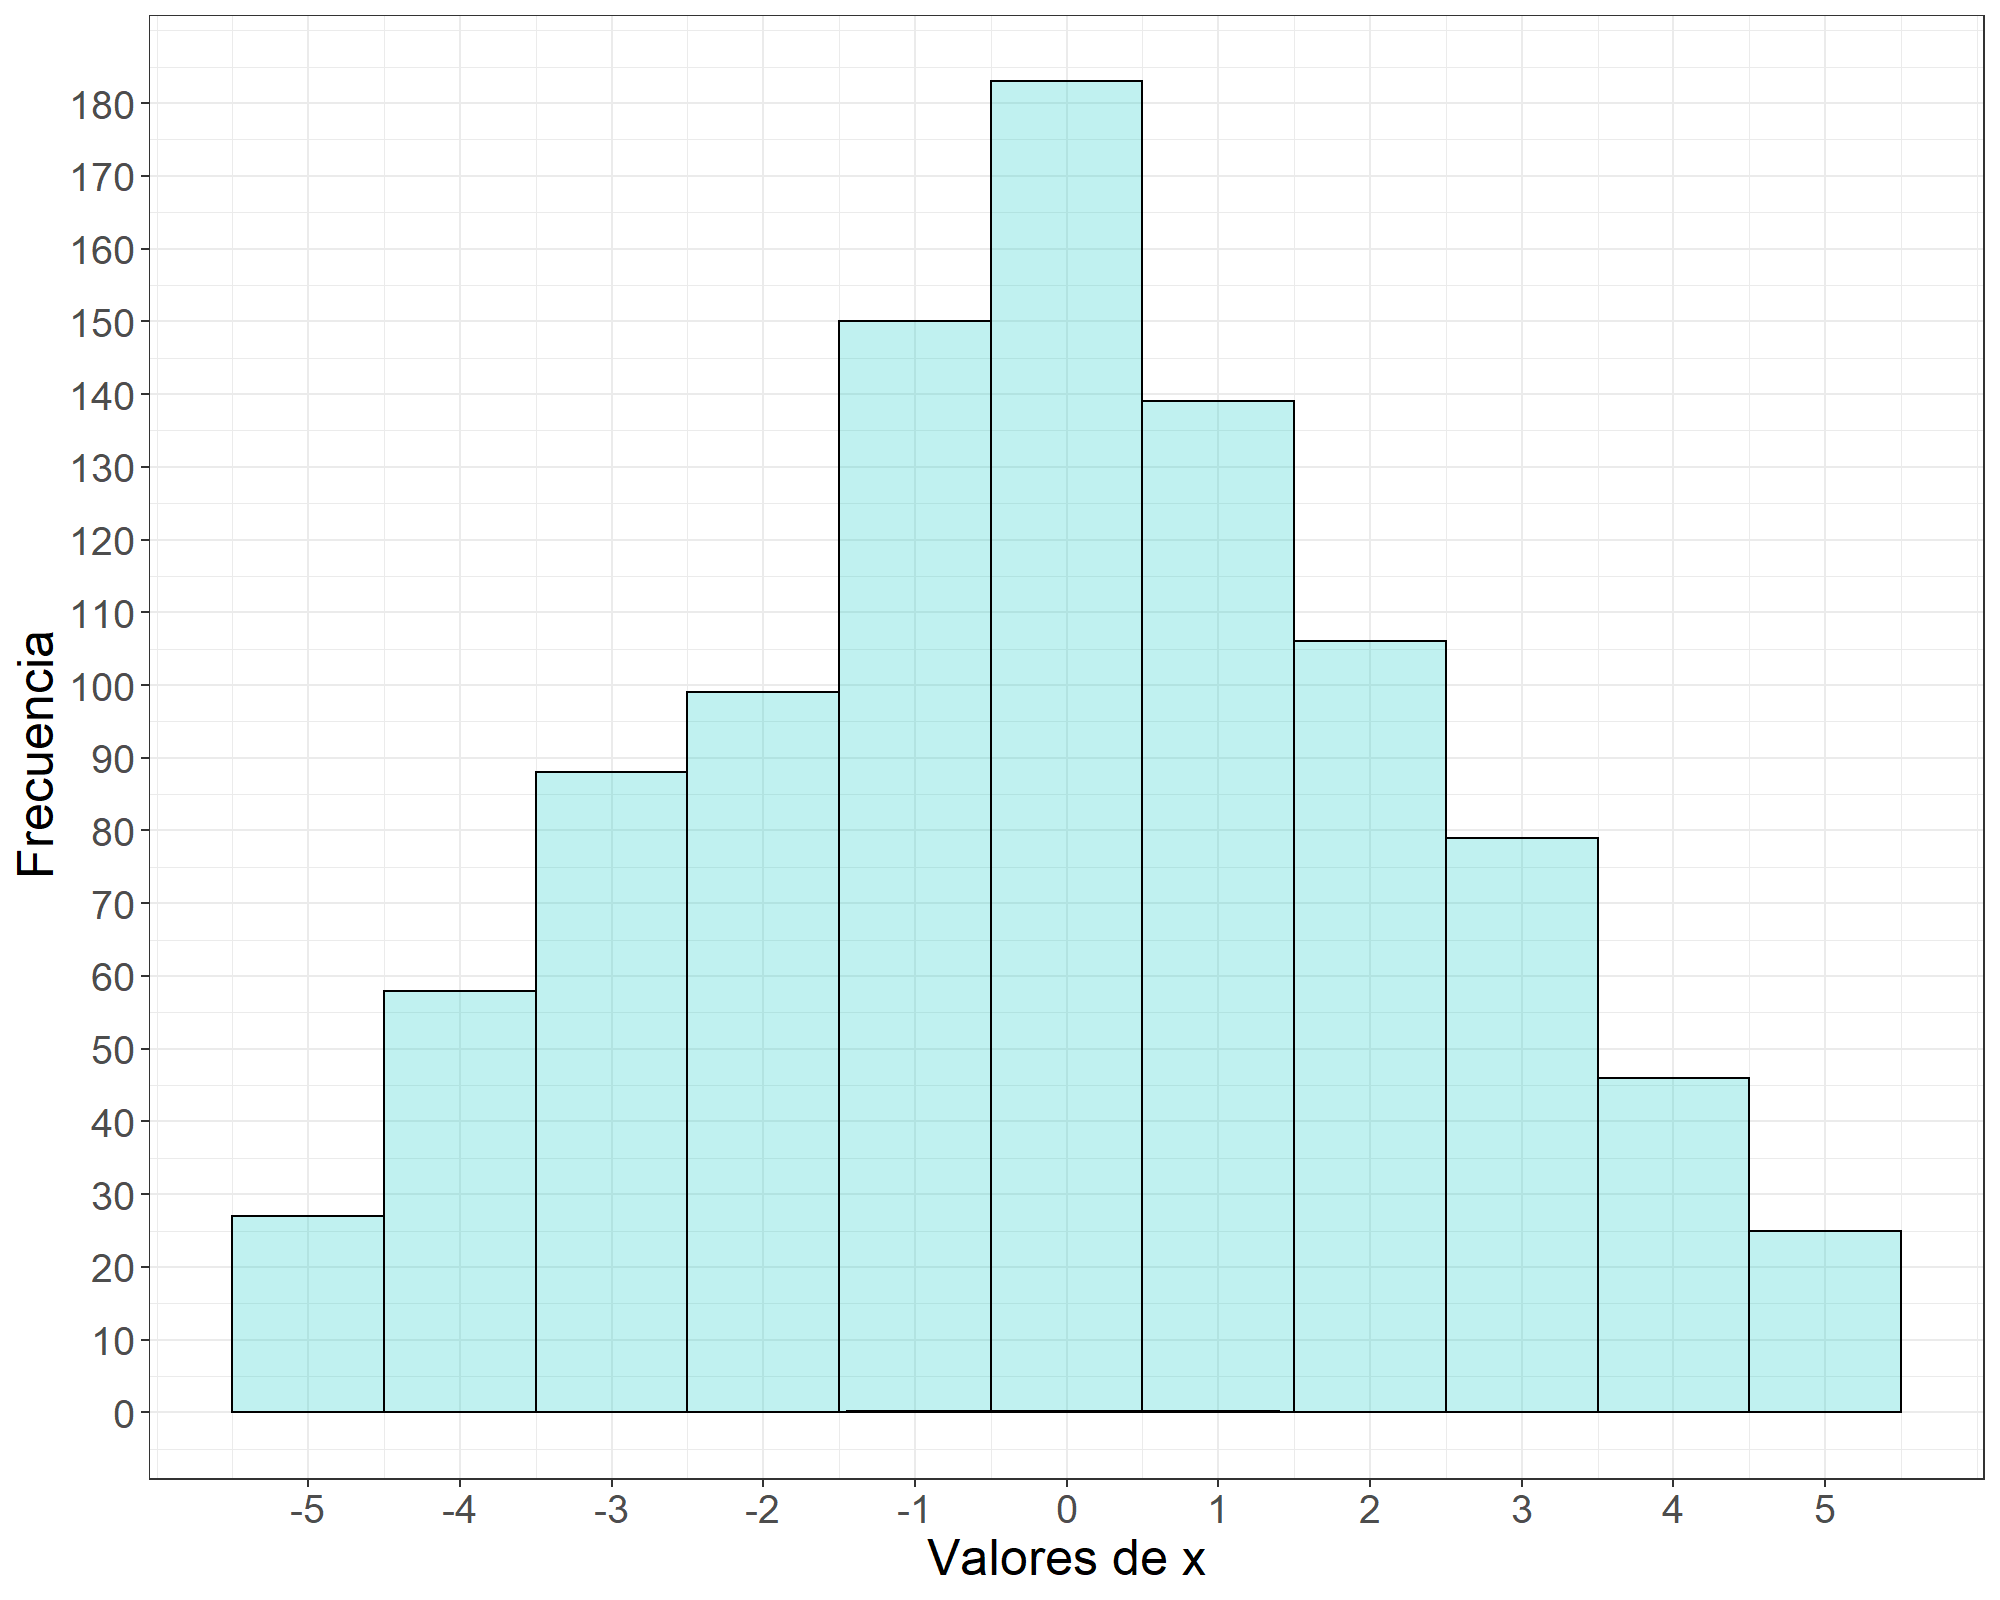
\includegraphics[scale=0.30]{figuras/restas.png}}
\label{fig:a}
\centering
\subfigure[Histograma de densidad de la variable aleatoria $Y$]{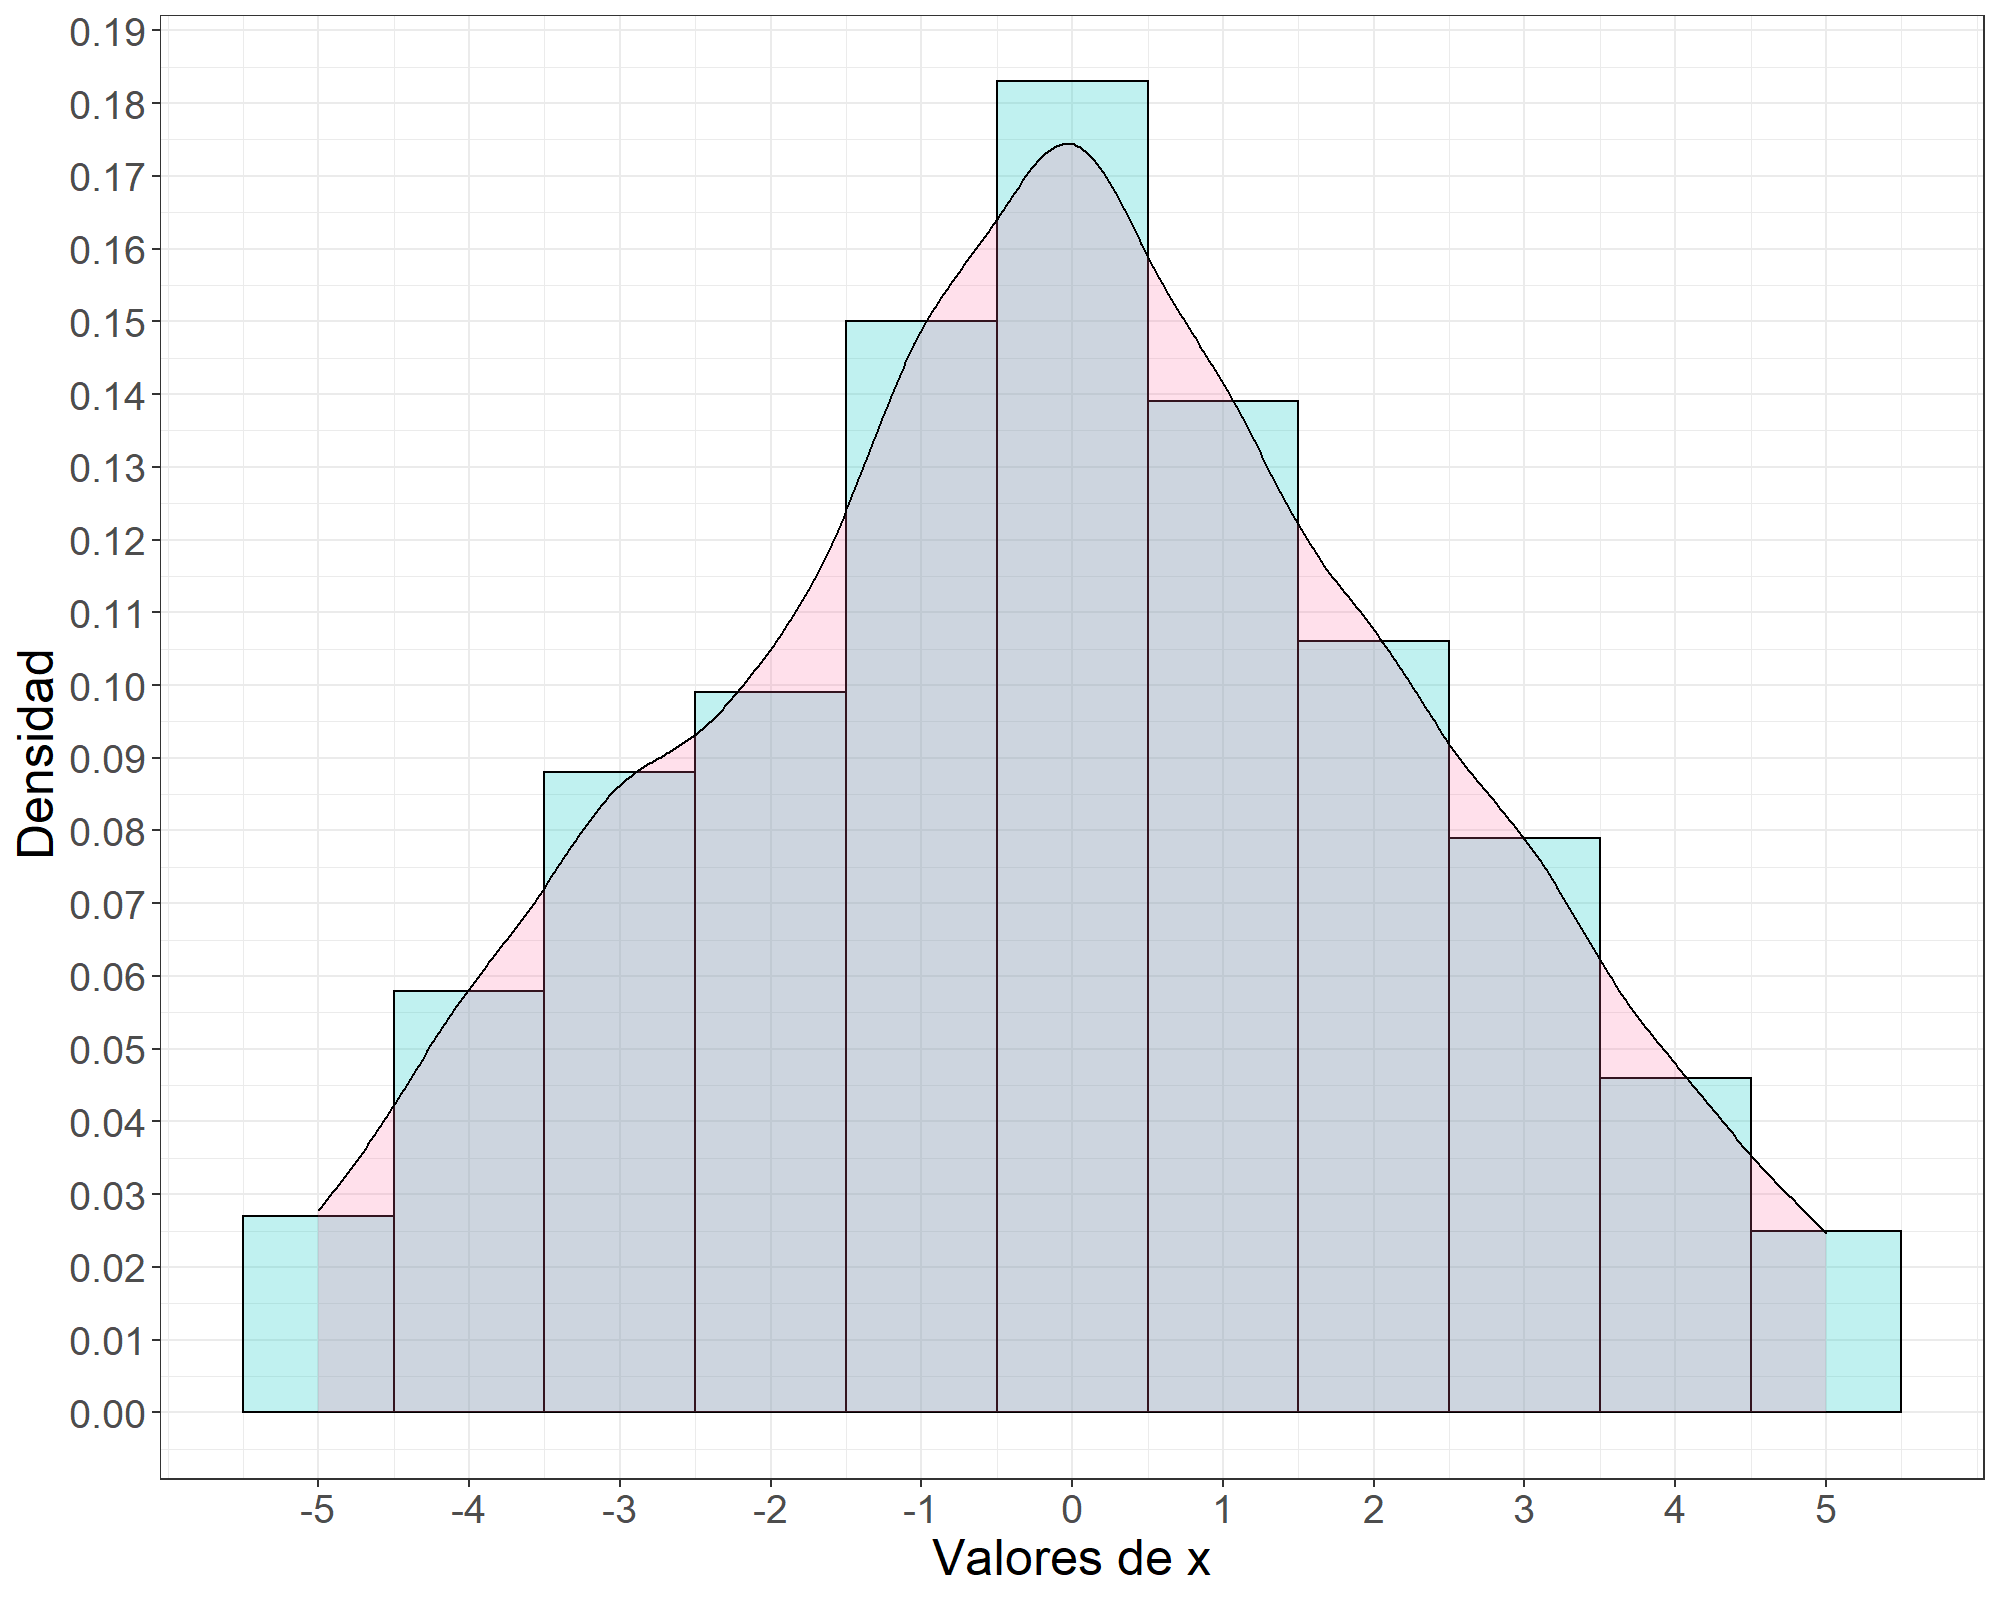
\includegraphics[scale=0.30]{figuras/drestas.png}}
\label{fig:s}
\centering
\caption{Histogramas de la variable aleatoria $Y = a - b$ }
\label{fig:2} 
\end{figure}

\subsection{$E(XY)= E((a+b)(a-b))$}
Dado que $E(XY)= E((a+b)(a-b))$, tenemos para $XY$ los valores que se muestran en el cuadro \ref{tab:3} de la página \pageref{tab:3}. 



\begin{table}[H]
  \centering
  \caption{Fragmento de valores de frecuencia de $XY$}
    \begin{tabular}{rrr}
    \toprule
    \multicolumn{1}{p{5.39em}}{\textbf{Posibles valores de \textit{\textbf{xy}}}} & \multicolumn{1}{l}{\textbf{frecuencia  \textit{\textbf{(xy)}}}}  & \multicolumn{1}{l}{\textit{\textbf{P(XY = xy)}}} \\
    \midrule
    -35   & 1     & 0.028 \\
    -32   & 1     & 0.028 \\
    -9    & 1     & 0.028 \\
    -8    & 1     & 0.028 \\
    -7    & 1     & 0.028 \\
    -5    & 1     & 0.028 \\
    -3    & 1     & 0.028 \\
    0     & 6     & 0.167 \\
    3     & 1     & 0.028 \\
    5     & 1     & 0.028 \\
    7     & 1     & 0.028 \\
    8     & 1     & 0.028 \\
    9     & 1     & 0.028 \\
    32    & 1     & 0.028 \\
    35    & 1     & 0.028 \\
    \bottomrule
    \end{tabular}%
  \label{tab:3}%
\end{table}%
Sustituyendo en la ecuación \ref{eq:3}
\begin{equation}
\begin{array}{ll}
   E[XY] &= \sum_{i=1}^{31} xy_{i}  \times P(XY=xy_{i})\\
   &\\
   E[XY] & = 0
  \end{array}
\end{equation}
Ahora para comprobar si $X$ e $Y$ son variables aleatorias independientes, hay que probar que se cumple para todos los casos se cumpla que $P(X,Y) = P(X)P(Y)$. Por lo anteriormente mencionado, con encontrar un caso donde no se cumpla la propiedad para decir que las variables aleatorias no son independientes. Como es el caso:
\begin{equation}
 P(X=12,Y=0) = P(a=6 , b=6) = \frac{1}{36} .  
\end{equation}
\begin{equation}
 P(X=12)P(Y=0) = \frac{1}{36} \times \frac{1}{6} = \frac{1}{216}.  
\end{equation}
Por tanto   $P(X=12,Y=0) \neq P(X=12)P(Y=0)$, lo que implica que $X$ e $Y$ no son variables aleatorias independientes.

Al realizar la simulación, los valores para la variable aleatoria $XY =(a+b)(a-b)$, los valores para $XY$ son almacenados en un \textit{dataframe}, como se muestra en el cuadro \ref{tab:m} de la página \pageref{tab:m}, al aplicarle la función \textit{summary} de R al \textit{dataframe} se obtiene los siguientes valores.  
\VerbatimInput{mult.txt}
\begin{table}[H]
  \centering
  \caption{Fragmento de \textit{dataframe} de la variable aleatoria $XY = (a+b)(a-b)$ }
    \begin{tabular}{rr}
    \toprule
    \multicolumn{1}{l}{Lanzamientos} & \multicolumn{1}{c}{xy} \\
    \midrule
    1     & -24 \\
    2     & -11 \\
    3     & -12 \\
    4     & -27 \\
    5     & 8 \\
    614   & 0 \\
    615   & -15 \\
    616   & 0 \\
    617   & -24 \\
    618   & 9 \\
    996   & 12 \\
    997   & -9 \\
    998   & 11 \\
    999   & -11 \\
    1000  & -5 \\
    \bottomrule
    \end{tabular}%
  \label{tab:m}%
\end{table}%

En los valores obtenidos se puede observar que la media es igual a -0.504 por lo que se puede decir que el valor promedio obtenido es similar a la $E[XY]$, además la $E[XY]$ coincide con la mediana que es el valor con mayor frecuencia de ocurrencia de $XY$ como se muestra en la figura \ref{fig:2} de la página \pageref{fig:2}. Para mejor visualización del experimento se puede ver la figura  \href{https://github.com/Albertomnoa/Tareas_MPA/blob/master/Tarea10/gif/multipli.gif}{$XY = (a+b)(a-b)$.gif}, donde se observa el progreso de los lanzamientos.

\begin{figure}[H]
\centering
\subfigure[Histograma de frecuencia de la variable aleatoria $XY$]{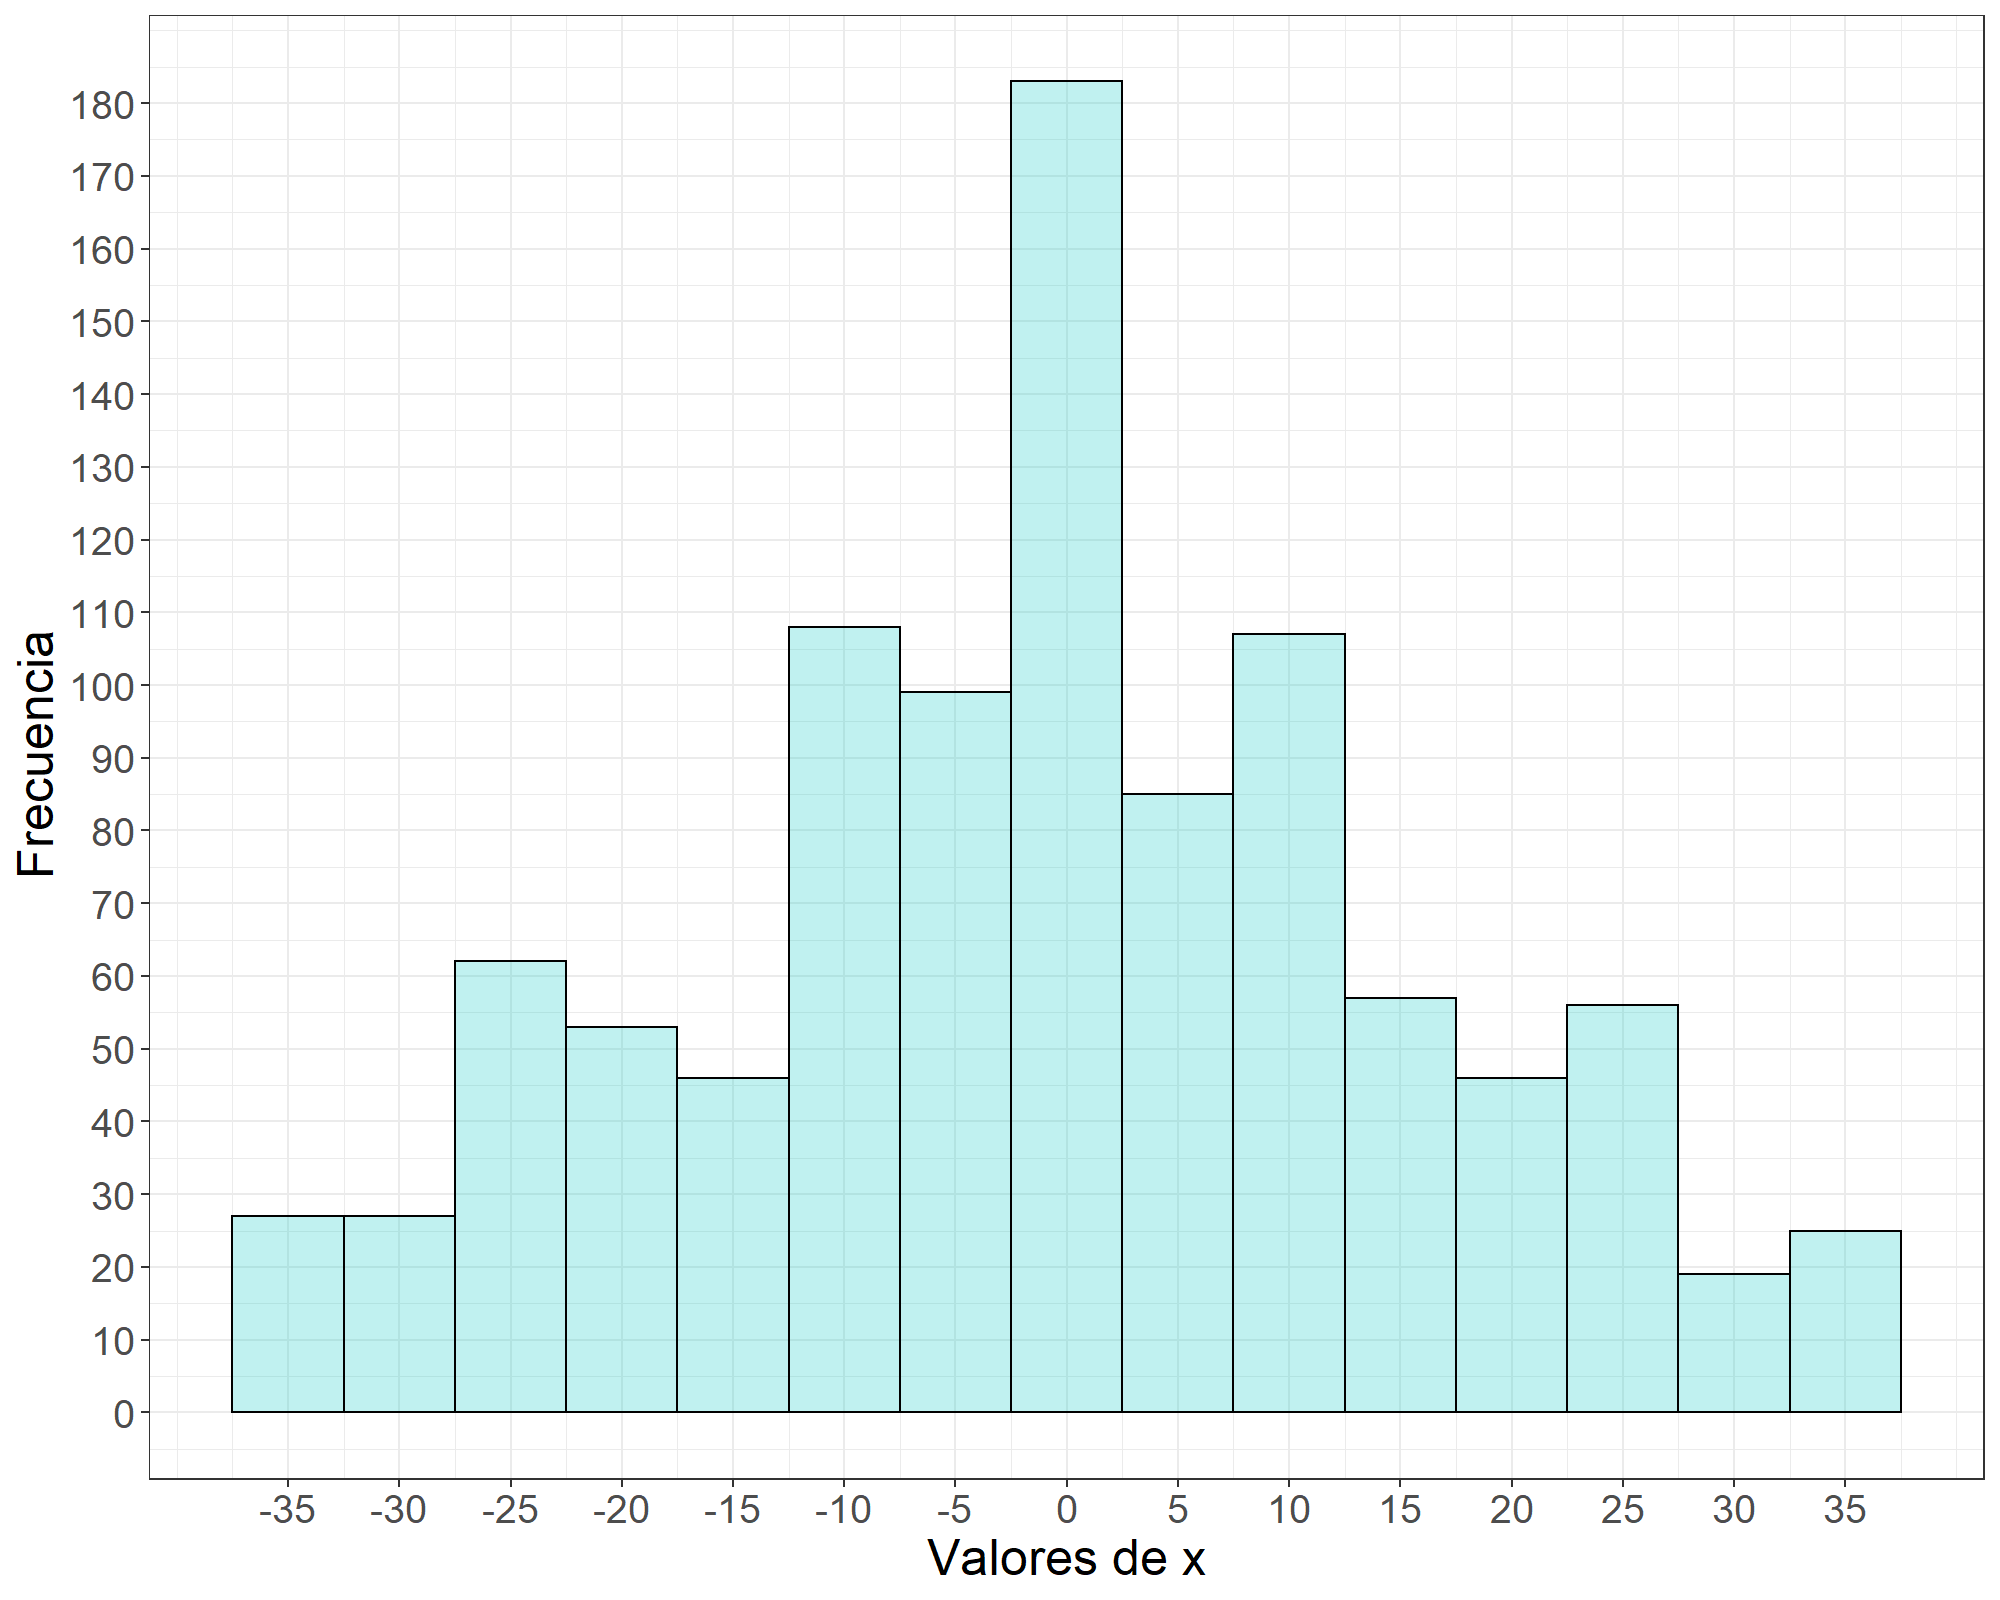
\includegraphics[scale=0.30]{figuras/mult.png}}
\label{fig:a}
\centering
\subfigure[Histograma de densidad de la variable aleatoria $XY$]{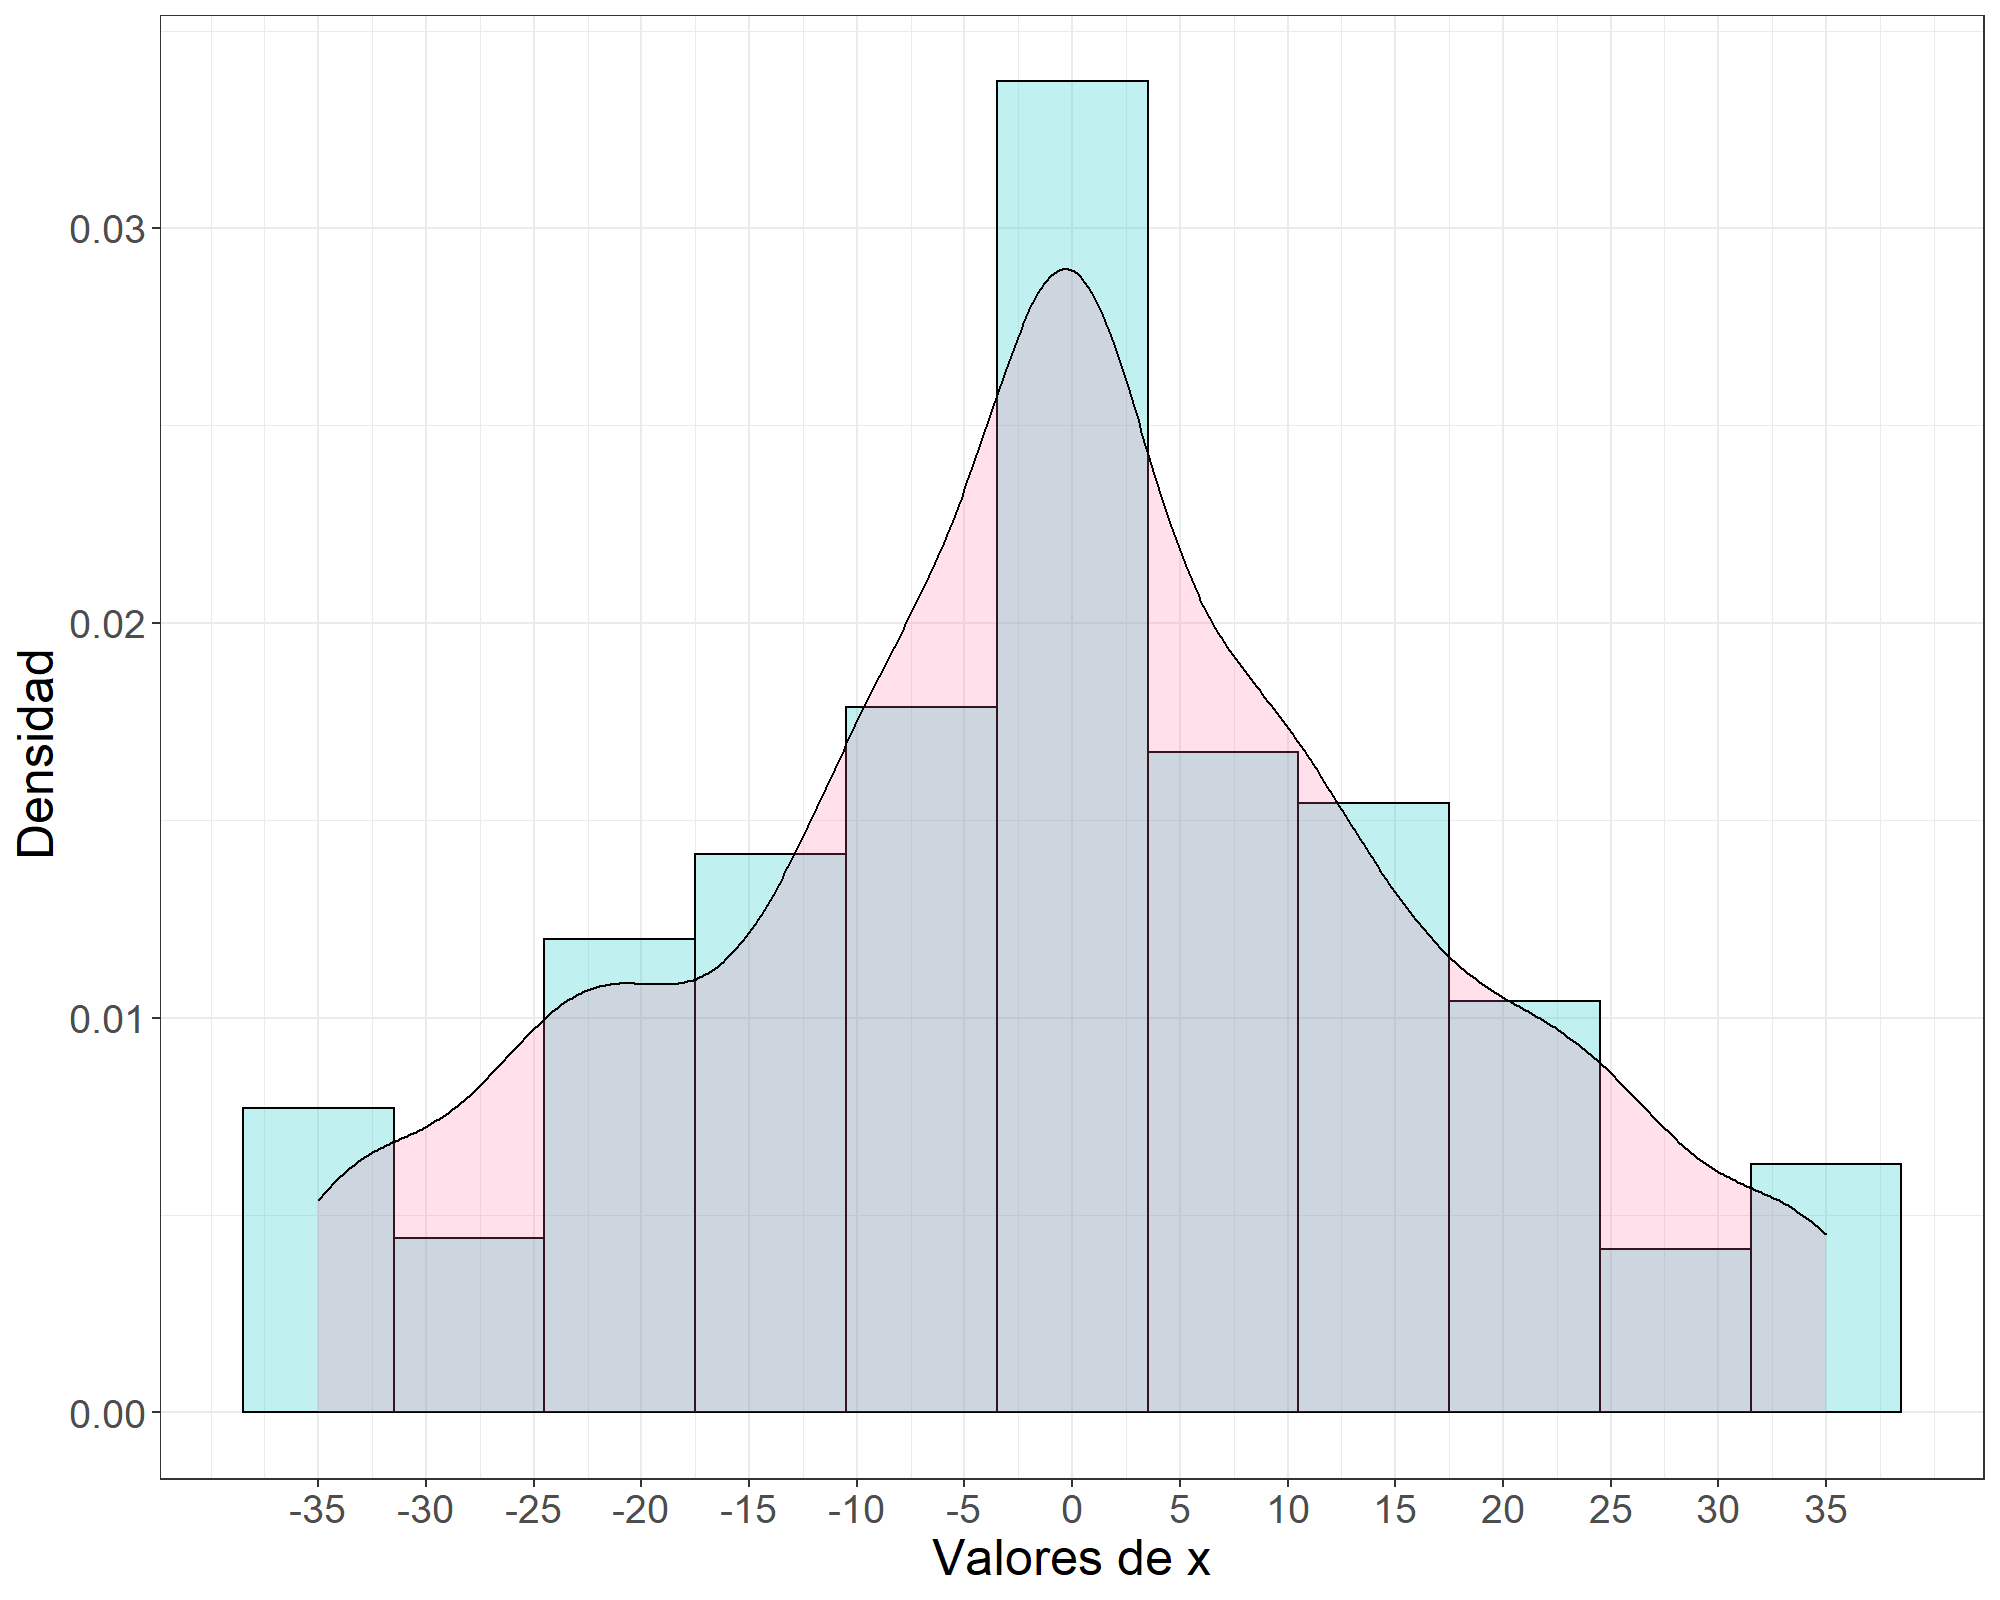
\includegraphics[scale=0.30]{figuras/dmult.png}}
\label{fig:s}
\centering
\caption{Histogramas de la variable aleatoria $XY = (a+b)(a-b)$ }
\label{fig:2} 
\end{figure}

Mediante la simulación se pudo constatar que los los resultados para la esperanza 

\section{Ejercicio 18 de la página 249}  
  
\emph{Exactly one of six similar keys opens a certain door. If you try the keys, one after another, what is the expected number of keys that you will have to try before success?}

\paragraph{Respuesta:} La variable aleatoria $X$ viene dada por el número de intentos fallidos antes de un éxito. Por lo que se tienen los valores en el cuadro \ref{tab:5} de la página \pageref{tab:5}.

\begin{table}[H]
  \centering
  \caption{Probabilidades de ocurrencia de $x$}
    \begin{tabular}{rr}
    \toprule
    \multicolumn{1}{l}{\textbf{\# de intentos ($x$)}} & \multicolumn{1}{c}{\textit{\textbf{P(X = x)}}} \\

    \midrule
    0     & $1/6$ \\
    1     & $(5/6) \times (1/5)= 1/6$ \\
    2     & $(5/6)\times(4/5)\times(1/4)= 1/6$ \\
    3     & $(5/6)\times(4/5)\times(3/4)\times(1/3)= 1/6$ \\
    4     & $(5/6)\times(4/5)\times(3/4)\times(2/3)\times(1/2)= 1/6$ \\
    5     & $(5/6)\times(4/5)\times(3/4)\times(2/3)\times(1/2)\times1= 1/6$ \\
    \bottomrule
    \end{tabular}%
  \label{tab:5}%
\end{table}%
Entonces se sustituye en la ecuación \ref{eq:3}:
\begin{equation}
\begin{array}{ll}
   E[X] &= 0\times \left(\frac{1}{6}\right) + 1\times \left(\frac{1}{6}\right)+ 2\times \left(\frac{1}{6}\right)+ 3\times \left(\frac{1}{6}\right)+ 4\times \left(\frac{1}{6}\right)+ 5\times \left(\frac{1}{6}\right) \\
   &\\
   E[X] & =\left(\frac{5}{2}\right). 
   
  \end{array}
\end{equation}
Por lo que el número esperado de intentos antes de abrir la puerta es 2.5.

Para la comprobación y mejor entendimiento del resultado obtenido se realiza una simulación de la variable aleatoria $X$, la misma es realizada por el código \ref{cod:2} a continuación.
\begin{center}
\lstinputlisting[ language=R, firstline=131, lastline=143]{Tarea10.R}
\label{cod:2}
\end{center}
Los valores para $X$ son almacenados en un \textit{dataframe}, como se muestra en el cuadro \ref{tab:p} de la página \pageref{tab:p}, al aplicarle la función \textit{summary} de R al \textit{dataframe} se obtiene los siguientes valores.  
\VerbatimInput{intentos.txt}

\begin{table}[H]
  \centering
  \caption{Fragmento de \textit{dataframe} con valores de $X$ obtenido en los experimentos}
    \begin{tabular}{rr}
    \toprule
    \multicolumn{1}{l}{Experimentos} & \multicolumn{1}{c}{X} \\
    \midrule
    1     & 3 \\
    2     & 5 \\
    3     & 3 \\
    4     & 3 \\
    5     & 5 \\
    177   & 5 \\
    178   & 0 \\
    179   & 0 \\
    180   & 1 \\
    181   & 1 \\
    996   & 3 \\
    997   & 3 \\
    998   & 2 \\
    999   & 4 \\
    1000  & 5 \\
    \bottomrule
    \end{tabular}%
  \label{tab:addlabel}%
\end{table}%

En los valores obtenidos se puede observar que la media es igual a 2.927 por lo que se puede decir que el valor promedio obtenido no es igual a la $E[X]$, además no coincide con la mediana ni con el valor de valor con mayor frecuencia de ocurrencia de $X$ que es cinco intentos. Lo anterior se muestra en la figura \ref{fig:p} de la página \pageref{fig:p}.

\begin{figure}[H]
\centering
\subfigure[Histograma de frecuencia de la variable aleatoria $X$]{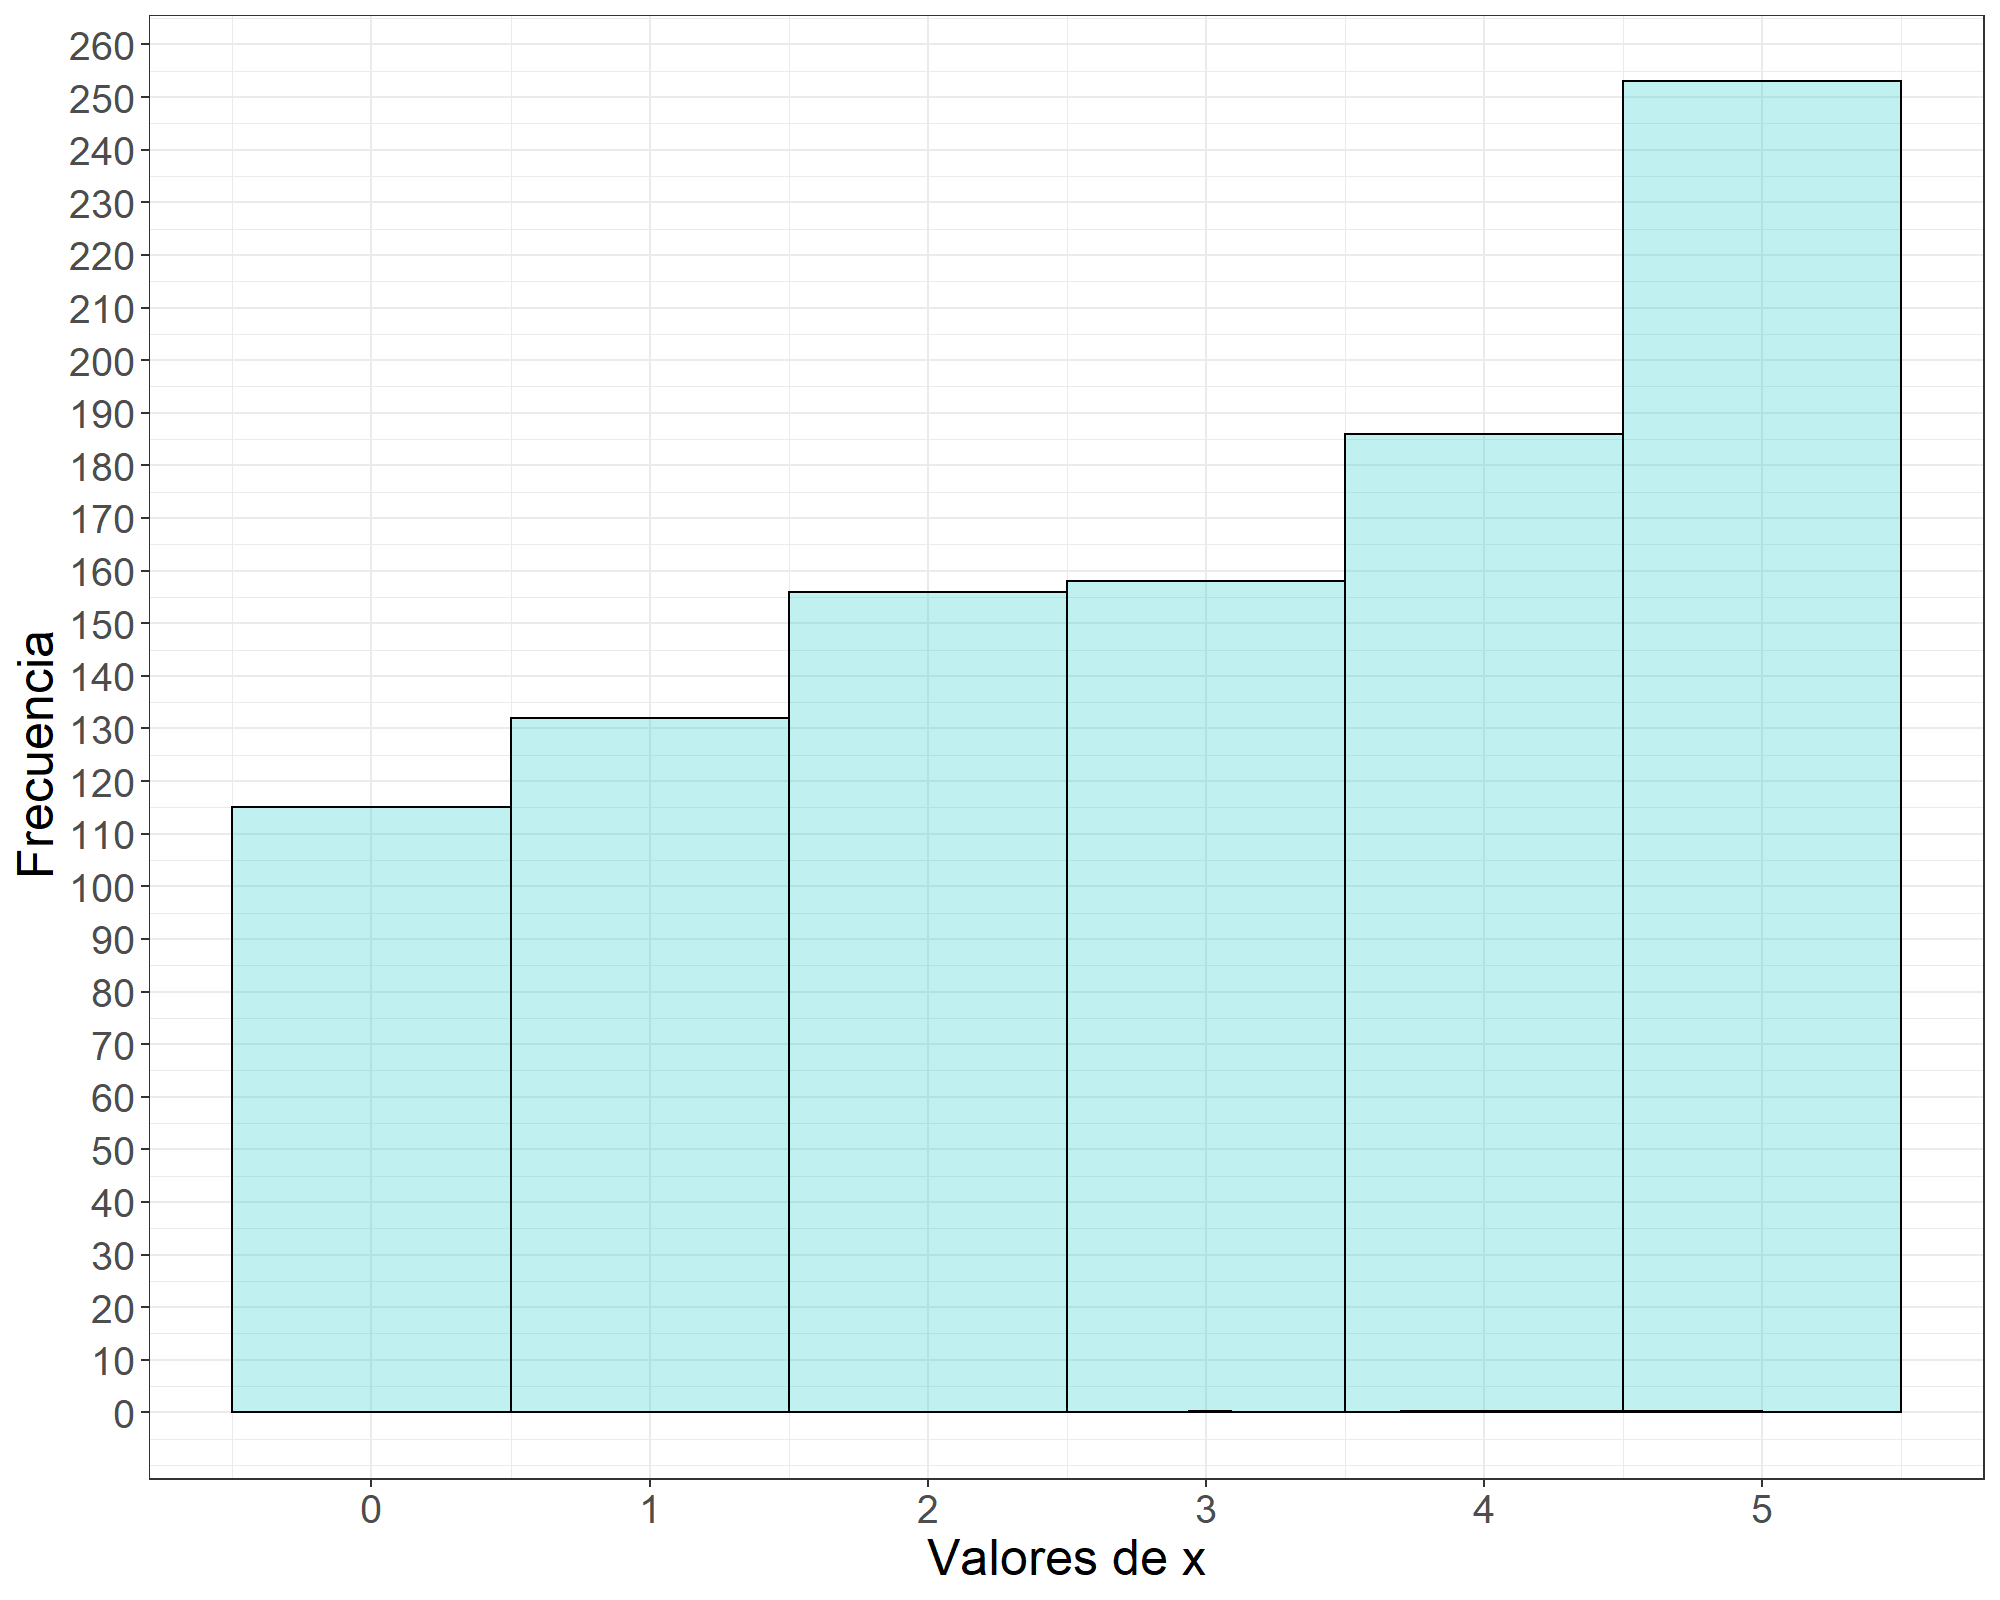
\includegraphics[scale=0.30]{figuras/intentos.png}}
\label{fig:a}
\centering
\subfigure[Histograma de densidad de la variable aleatoria $X$]{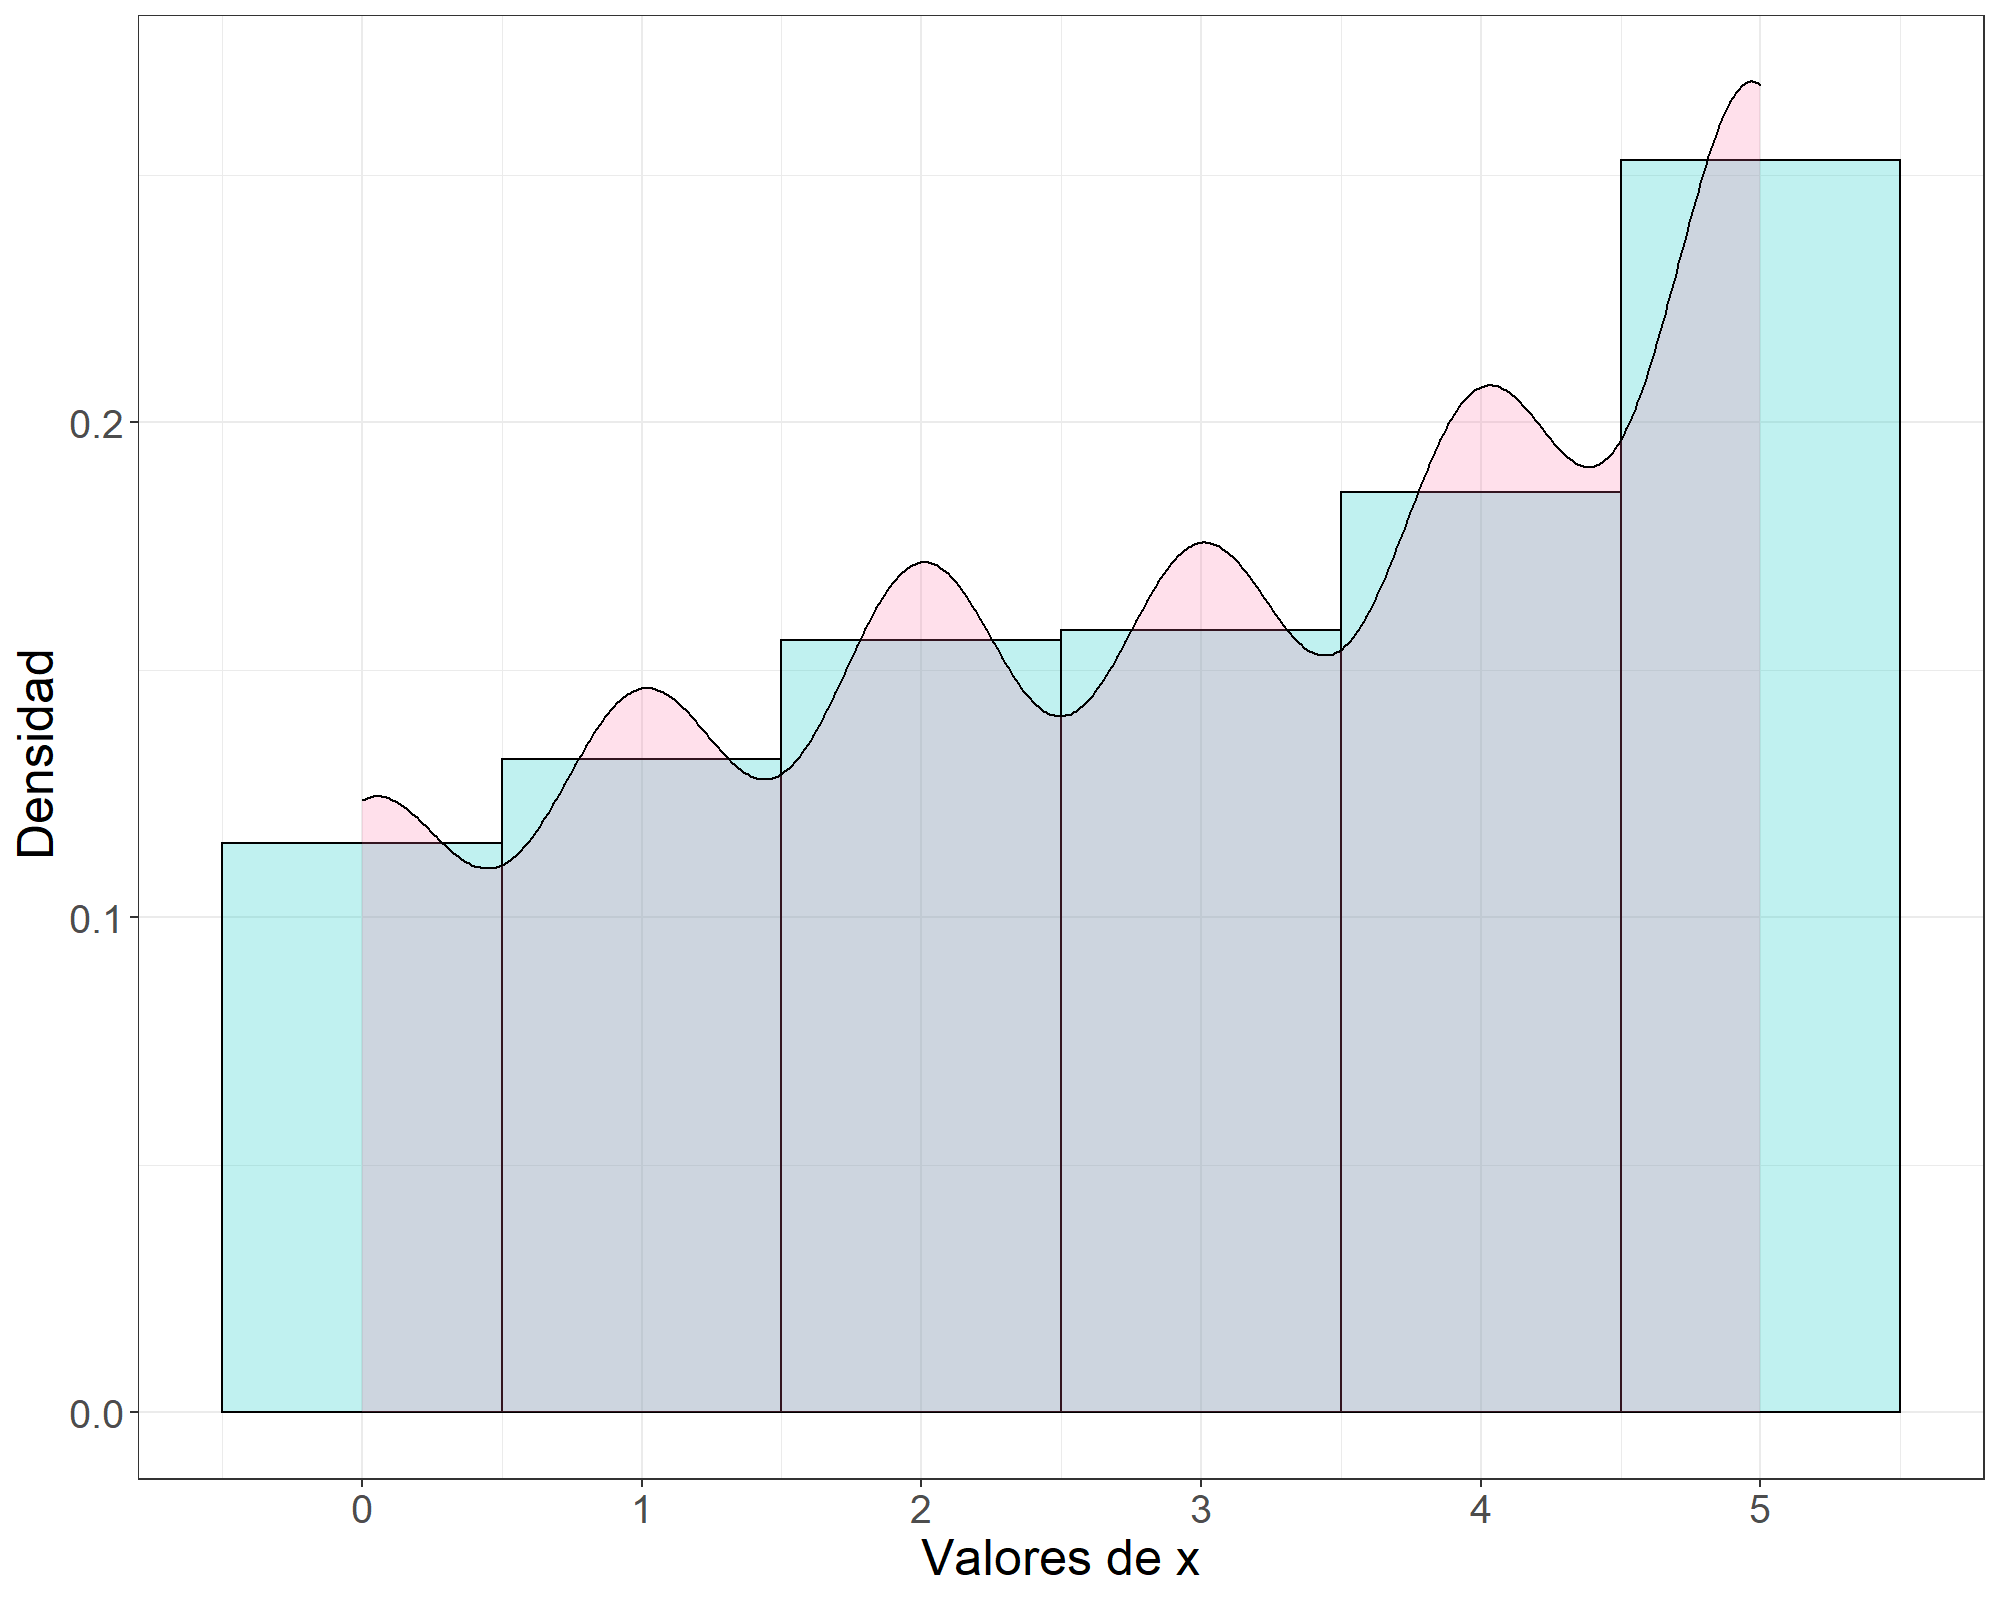
\includegraphics[scale=0.30]{figuras/dintentos.png}}
\label{fig:s}
\centering
\caption{Histogramas de la variable aleatoria $X$ }
\label{fig:p} 
\end{figure}
Con los valores numéricos obtenidos en la simulación se llega a una contradicción a los resultados obtenidos de forma analítica. 

\section{Ejercicio 19 de la página 249}  
\emph{A multiple choice exam is given. A problem has four possible answers, and exactly one answer is correct. The student is allowed to choose a subset of the four possible answers as his answer. If his chosen subset contains the correct answer, the student receives three points, but he loses one point for each wrong answer in his chosen subset. Show that if he just guesses a subset uniformly and randomly his expected score is zero.}

\paragraph{Respuesta:} Sea la puntuación obtenida en la elección del subconjunto de posibles respuestas una variable aleatoria $X$, se tiene que el espacio muestral está conformado por dieciséis formas de escoger un subconjunto.  En el cuadro \ref{tab:6} de la página \pageref{tab:6} se muestra la cardinalidad de los posibles subconjuntos, así como los posibles valores de $x$ y las probabilidades asociadas a dichos valores.
\begin{table}[H]
  \centering
  \caption{Cardinalidad de los subconjunto con  sus posibles valores y probabilidades}
    \begin{tabular}{crr}
    \toprule
    \multicolumn{1}{p{7em}}{\textbf{Elementos de Subconjuntos}} & \multicolumn{1}{p{5.39em}}{\textbf{Posibles Valores de \textit{\textbf{x}}}} & \multicolumn{1}{c}{\textit{\textbf{P(X = x)}}} \\
    \midrule
    0     & 0     & 1/16 \\
    \midrule
    \multirow{2}[2]{*}{1} & 3     & 1/16 \\
          & -1    & 3/16 \\
    \midrule
    \multirow{2}[2]{*}{2} & 2     & 3/16 \\
          & -2    & 3/16 \\
    \midrule
    \multirow{2}[2]{*}{3} & 1     & 3/16 \\
          & -3    & 1/16 \\
    \midrule
    4     & 0     & 1/16 \\
    \bottomrule
    \end{tabular}%
  \label{tab:6}%
\end{table}%

Sustituyendo en la ecuación \ref{eq:3}:
\begin{equation}
\begin{array}{ll}
   E[X] &= 3\times \left(\frac{1}{16}\right) - 1\times \left(\frac{3}{16}\right)+ 2\times \left(\frac{3}{16}\right)- 2\times \left(\frac{3}{16}\right)+ 1\times \left(\frac{3}{16}\right)- 3\times \left(\frac{1}{16}\right) \\
   &\\
   E[X] & = 0. 
  
   \end{array}
   \end{equation}
    Entonces si solo adivina un subconjunto de manera uniforme y aleatoria, su puntuación esperada es cero.
    
Para la comprobación y mejor entendimiento del resultado obtenido se realiza una simulación de la variable aleatoria $X$, la misma es realizada por el código \ref{cod:2} a continuación.
\begin{center}
\lstinputlisting[ language=R, firstline=166, lastline=197]{Tarea10.R}
\label{cod:2}
\end{center}
Los valores para $X$ son almacenados en un \textit{dataframe}, como se muestra en el cuadro \ref{tab:p} de la página \pageref{tab:p}, al aplicarle la función \textit{summary} de R al \textit{dataframe} se obtiene los siguientes valores.  
\VerbatimInput{es.txt}
\begin{table}[H]
  \centering
  \caption{Fragmento}
    \begin{tabular}{rr}
    \toprule
    \multicolumn{1}{l}{Experimentos} & \multicolumn{1}{c}{x} \\
    \midrule
    1     & 3 \\
    2     & -2 \\
    3     & -2 \\
    4     & -3 \\
    5     & -3 \\
    6     & -3 \\
    7     & 3 \\
    8     & -2 \\
    9     & -2 \\
    10    & 1 \\
    5996  & -2 \\
    5997  & -2 \\
    5998  & -3 \\
    5999  & -3 \\
    6000  & 1 \\
    \bottomrule
    \end{tabular}%
  \label{tab:addlabel}%
\end{table}%
En los valores obtenidos se puede observar que la media es igual a -2 por lo que se puede decir que el valor promedio es negativo por lo que se puede decir que va a obtener cero en el examen.
 El código general se encuentra disponible en el repositorio. \href{https://github.com/Albertomnoa/Tareas_MPA/tree/master/Tarea10}{https://github.com/Albertomnoa/Tareas} \textbf{} 

   
\newpage
\bibliographystyle{plain}
\bibliography{Biblio}

\end{document}
